\documentclass[../mathNotesPreamble]{subfiles}

\begin{document}
%  \relscale{1.4} %TODO
  \section{6.2: The Normal Model}
    \begin{defn*}
      The \textbf{Normal Distribution} is a symmetric, unimodal model that provides a very close fit for many numerical variables:
      \[\frac{1}{\sigma\sqrt{2\pi}} e^{-\frac{1}{2}\parens{\frac{x-\mu}{\sigma}}^2}\]
      We use $N(\mu,\sigma)$ to denote the Normal Distribution with mean $\mu$ and standard deviation $\sigma$. \\
      \emph{Note:}
        \begin{itemize}
          \item $\mu$ and $\sigma$ are used in the context of a probability distribution, whereas $\overline{x}$ and $s$ are used for data.
          \item Other sources denote the Normal Distribution with mean $\mu$ and \emph{variance} $\sigma^2$ as $N(\mu,\sigma^2)$ or $\mathcal{N}(\mu,\sigma^2)$.
        \end{itemize}
    \end{defn*}
    \vspace*{\stretch{1}}

    \begin{ex*}
      Below are some histograms from a dataset that show the measured cholesterol and diastolic blood pressure from 2,793 people. These histograms have the Normal Distribution with the corresponding mean $\mu$ and standard deviation $\sigma$ overlayed:
    \end{ex*}
    \begin{center}
      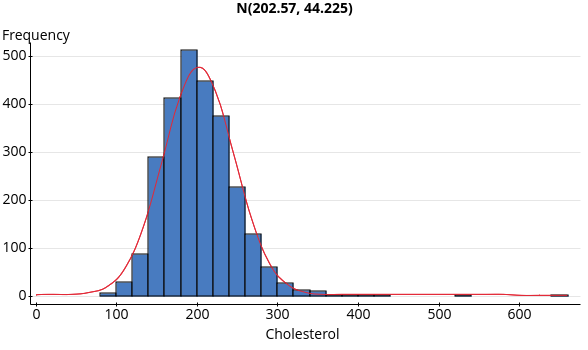
\includegraphics[width=0.49\linewidth]{images/math211_figure_6p9a}
      \hspace*{\stretch{1}}
      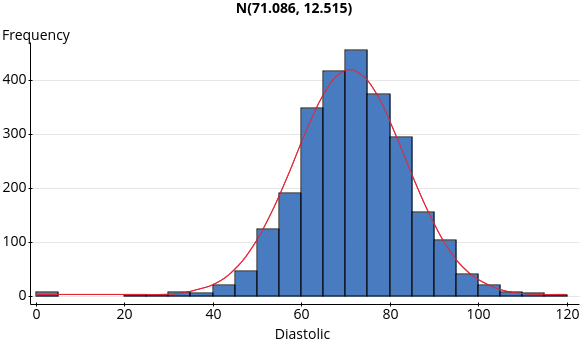
\includegraphics[width=0.49\linewidth]{images/math211_figure_6p9b}%\\[\baselineskip]
%
%      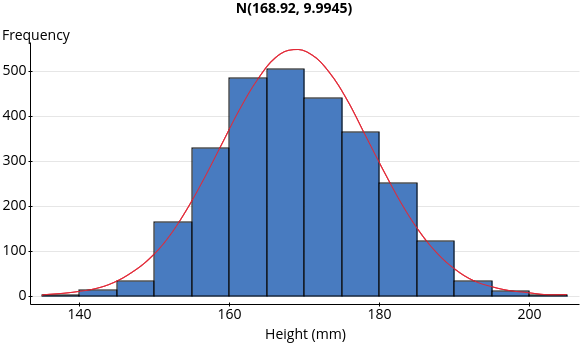
\includegraphics[width=0.475\linewidth]{images/math211_figure_6p9c}
%
    \end{center}
    \pagebreak

    \begin{ex*}
      Below is the graph of two Normal Distributions with equal means, but different standard deviations.
    \end{ex*}
    \begin{center}
      \begin{tikzpicture}[scale=1.0, declare function={
        N=50;
        mu=10; sig=3.0;
        xmin=mu-3.2*sig;
        xmax=mu+3.2*sig;
        ymin=-0.1*gauss(mu,mu,sig);
        h=0.08*gauss(mu,mu,sig);}]

        \begin{axis}[
          every axis plot post/.append style={
          mark=none, domain={xmin}:{xmax},samples=N,smooth},
          axis lines=center,
          ymin=ymin,
          axis line style={black,->},
          every axis x label/.style={at={(current axis.right of origin)},anchor=north},
          xlabel=Values, xlabel style={at={(axis description cs:0.5,-0.125)},anchor=north},
          ylabel=Density, ylabel style={at={(axis description cs:-0.075,0.5)},rotate=90,anchor=south},
          width=0.9*\textwidth, height=0.325*\textwidth,
          clip=false,
          ]

          % PLOTS
          \addplot[lander_blue,thick] {gauss(x,mu,sig)} node[pos=0.675, above right, black, fill=white, opacity=0.0, text opacity=1.0, font=\normalsize, align=left] {Larger\\ standard\\ deviation};
          \addplot[red,thick] {gauss(x,mu,sig/2)} node[pos=0.55, above right, black, fill=white, opacity=0.0, text opacity=1.0, font=\normalsize, align=left] {Smaller\\ standard\\ deviation};
        \end{axis}
      \end{tikzpicture}
    \end{center}
    \vspace*{\stretch{1}}
    
    \begin{ex*}
      Below is the graph of two Normal Distributions with equal standard deviations, but different means.
    \end{ex*}
    \begin{center}
      \begin{tikzpicture}[scale=1.0, declare function={
        N=50;
        mu=64; sig=3.0;
        mu_shift=5;
        xmin=mu-3.2*sig;
        xmax=mu+3.2*sig;
        ymin=-0.1*gauss(mu,mu,sig);
        h=0.08*gauss(mu,mu,sig);}]

        \begin{axis}[
          scaled ticks=false,
          /pgf/number format/.cd, fixed, precision=2, %forces large ytick labels
          every axis plot post/.append style={
          mark=none,samples=N,smooth},
          axis lines=center,
          ymin=ymin,
          axis line style={black,->},
          every axis x label/.style={at={(current axis.right of origin)},anchor=north},
          xlabel=Height (inches), xlabel style={at={(axis description cs:0.5,-0.125)},anchor=north},
          ylabel=Density, ylabel style={at={(axis description cs:-0.075,0.5)},rotate=90,anchor=south},
          width=0.9*\textwidth, height=0.325*\textwidth,
          clip=false,
          ]

          % PLOTS
          \addplot[lander_blue,thick, domain=xmin:xmax] {gauss(x,mu,sig)} node[pos=0.35, above left, black, fill=white, opacity=0.0, text opacity=1.0, font=\normalsize, align=left] {Women};
          \addplot[red,thick, domain={xmin+mu_shift}:{xmax+mu_shift}] {gauss(x,mu+mu_shift,sig)} node[pos=0.65, above right, black, fill=white, opacity=0.0, text opacity=1.0, font=\normalsize, align=left] {Men};
        \end{axis}
      \end{tikzpicture}
    \end{center}
    \vspace*{\stretch{1}}
    What is the area under each of the curves above?
    \vspace*{\stretch{1}}
  \pagebreak

  \begin{ex*}
    Suppose that the Normal model $N(64,3)$ gives a good approximation to the distribution of adult women's height in the United States. If a women is chosen at random, what is the probability that
  \end{ex*}
  \begin{extasks}[after-item-skip=\stretch{1}](1)
    \task she is taller than 62''?

      \begin{tikzpicture}[scale=1.0, declare function={
        N=50;
        mu=64; sig=3.0;
        xmin=mu-3.2*sig;
        xmax=mu+3.2*sig;
        ymin=-0.1*gauss(mu,mu,sig);
        h=0.08*gauss(mu,mu,sig);}]

        \begin{axis}[
          scaled ticks=false,
          /pgf/number format/.cd, fixed, precision=2, %forces large ytick labels
          every axis plot post/.append style={
          mark=none, domain={xmin}:{xmax},samples=N,smooth},
          axis lines=center,
          ymin=ymin, ymajorticks=false,
          axis line style={black,->},
          every axis x label/.style={at={(current axis.right of origin)},anchor=north},
          xlabel=Height (inches), xlabel style={at={(axis description cs:0.5,-0.0625)},anchor=north},
          ylabel=Density, ylabel style={at={(axis description cs:-0.025,0.5)},rotate=90,anchor=south},
          width=0.5*\textwidth, height=0.325*\textwidth,
          clip=false,
          ]

          % PLOTS
          \addplot[lander_blue,thick, name path=B] {gauss(x,mu,sig)};
            
          % FILL
          \path[name path=xaxis]
            (\pgfkeysvalueof{/pgfplots/xmin},0) -- (\pgfkeysvalueof{/pgfplots/xmax},0);
          \addplot[lander_blue!50] fill between[of=xaxis and B, soft clip={domain=62:{mu+3*sig}}];
          \addplot[draw=black] (62,0) -- (62,{gauss(62,mu,sig)});
        \end{axis}
      \end{tikzpicture}
    \task she is shorter than 62''?

      \begin{tikzpicture}[scale=1.0, declare function={
        N=50;
        mu=64; sig=3.0;
        xmin=mu-3.2*sig;
        xmax=mu+3.2*sig;
        ymin=-0.1*gauss(mu,mu,sig);
        h=0.08*gauss(mu,mu,sig);}]

        \begin{axis}[
          scaled ticks=false,
          /pgf/number format/.cd, fixed, precision=2, %forces large ytick labels
          every axis plot post/.append style={
          mark=none, domain={xmin}:{xmax},samples=N,smooth},
          axis lines=center,
          ymin=ymin, ymajorticks=false,
          axis line style={black,->},
          every axis x label/.style={at={(current axis.right of origin)},anchor=north},
          xlabel=Height (inches), xlabel style={at={(axis description cs:0.5,-0.0625)},anchor=north},
          ylabel=Density, ylabel style={at={(axis description cs:-0.025,0.5)},rotate=90,anchor=south},
          width=0.5*\textwidth, height=0.325*\textwidth,
          clip=false,
          ]

          % PLOTS
          \addplot[lander_blue,thick, name path=B] {gauss(x,mu,sig)};
            
          % FILL
          \path[name path=xaxis]
            (\pgfkeysvalueof{/pgfplots/xmin},0) -- (\pgfkeysvalueof{/pgfplots/xmax},0);
          \addplot[lander_blue!50] fill between[of=xaxis and B, soft clip={domain={mu-3*sig}:62}];
          \addplot[draw=black] (62,0) -- (62,{gauss(62,mu,sig)});
        \end{axis}
      \end{tikzpicture}
  \end{extasks}
  \vspace*{\stretch{1}}
  \pagebreak
  \begin{extasks}[after-item-skip=\stretch{1}](1)
    \task her height is between 62'' and 67''?

      \begin{tikzpicture}[scale=1.0, declare function={
        N=50;
        mu=64; sig=3.0;
        xmin=mu-3.2*sig;
        xmax=mu+3.2*sig;
        ymin=-0.1*gauss(mu,mu,sig);
        h=0.08*gauss(mu,mu,sig);}]

        \begin{axis}[
          scaled ticks=false,
          /pgf/number format/.cd, fixed, precision=2, %forces large ytick labels
          every axis plot post/.append style={
          mark=none, domain={xmin}:{xmax},samples=N,smooth},
          axis lines=center,
          ymin=ymin, ymajorticks=false,
          axis line style={black,->},
          every axis x label/.style={at={(current axis.right of origin)},anchor=north},
          xlabel=Height (inches), xlabel style={at={(axis description cs:0.5,-0.0625)},anchor=north},
          ylabel=Density, ylabel style={at={(axis description cs:-0.025,0.5)},rotate=90,anchor=south},
          width=0.5*\textwidth, height=0.325*\textwidth,
          clip=false,
          ]

          % PLOTS
          \addplot[lander_blue,thick, name path=B] {gauss(x,mu,sig)};
            
          % FILL
          \path[name path=xaxis]
            (\pgfkeysvalueof{/pgfplots/xmin},0) -- (\pgfkeysvalueof{/pgfplots/xmax},0);
          \addplot[lander_blue!50] fill between[of=xaxis and B, soft clip={domain=62:67}];
          \addplot[draw=black] (62,0) -- (62,{gauss(62,mu,sig)}) (67,0) -- (67,{gauss(67,mu,sig)});
        \end{axis}
      \end{tikzpicture}
  \end{extasks}
  \vspace*{\stretch{1}}
  
  \begin{ex*}
    ``Verify'' the emperical rule by using technology to find the probability that an observation lies within 1, 2, and 3 standard deviations.
  \end{ex*}
  \begin{center}
      %% Adapted from https://tikz.net/gaussians/
      % GAUSSIANs: 68-95-99 rule
      \begin{tikzpicture}[scale=1.0, declare function={
        N=50;
        mu=11; sig=3.0;
        xmin=mu-3.2*sig;
        xmax=mu+3.2*sig;
        ymin=-0.1*gauss(mu,mu,sig);
        h=0.08*gauss(mu,mu,sig);}]

        \begin{axis}[
          every axis plot post/.append style={
          mark=none,domain={mu-1.08*xmax/2}:{1.08*xmax},samples=N,smooth},
          xmin=xmin, xmax=xmax,
          axis x line=middle,
          ymin=ymin, ymax={1.1*gauss(mu,mu,sig)},
          axis y line=none,
          axis line style={thick, <->},
          enlargelimits=true,
          ticks=none,
          every axis x label/.style={at={(current axis.right of origin)},anchor=north},
          width=0.9*\textwidth, height=0.35*\textwidth,
          clip=false
          ]

          % PLOTS
          \addplot[lander_blue,thick,name path=B] {gauss(x,mu,sig)};
%
%          % FILL
          \path[name path=xaxis]
            (\pgfkeysvalueof{/pgfplots/xmin},0) -- (\pgfkeysvalueof{/pgfplots/xmax},0); %\pgfkeysvalueof{/pgfplots/xmin}
          \addplot[lander_blue!50] fill between[of=xaxis and B, soft clip={domain={mu-3*sig}:{mu+3*sig}}];
          \addplot[lander_blue!25] fill between[of=xaxis and B, soft clip={domain={mu-2*sig}:{mu+2*sig}}];
          \addplot[lander_blue!10] fill between[of=xaxis and B, soft clip={domain={mu-1*sig}:{mu+1*sig}}];

%          % LINES
          \addplot[black,dashed,thick]
            coordinates {({mu-3*sig},{20*gauss(mu-3*sig,mu,sig)}) ({mu-3*sig},{-h})}
            node[below=-3pt,scale=0.8] {\strut $\mu-3\sigma$};
          \addplot[black,dashed,thick]
            coordinates {({mu-2*sig},{4*gauss(mu-2*sig,mu,sig)}) ({mu-2*sig},{-h})}
            node[below=-3pt,scale=0.8] {\strut $\mu-2\sigma$};
          \addplot[black,dashed,thick]
            coordinates {({mu-1*sig},{1.3*gauss(mu-sig,mu,sig)}) ({mu-1*sig},{-h})}
            node[below=-3pt,scale=0.8] at ({mu-sig},{-h}) {\strut $\mu-\sigma$};
          \addplot[black,dashed,line width=0.7pt]
            coordinates {(mu,{1.05*gauss(mu,mu,sig)}) (mu,{-h})}
            node[below=-3pt,scale=0.8] {\strut $\mu$};
          \addplot[black,dashed,thick]
            coordinates {({mu+1*sig},{1.3*gauss(mu+sig,mu,sig)}) ({mu+1*sig},{-h})}
            node[below=-3pt,scale=0.8] at ({mu+sig},{-h}) {\strut $\mu+\sigma$};
          \addplot[black,dashed,thick]
                  coordinates {({mu+2*sig},{4*gauss(mu+2*sig,mu,sig)}) ({mu+2*sig},{-h})}
            node[below=-3pt,scale=0.8] at ({mu+2*sig},{-h}) {\strut $\mu+2\sigma$};
          \addplot[black,dashed,thick]
            coordinates {({mu+3*sig},{20*gauss(mu+3*sig,mu,sig)}) ({mu+3*sig},{-h})}
            node[below=-3pt,scale=0.8] at ({mu+3*sig},{-h}) {\strut $\mu+3\sigma$};

          % AREAS
          \addplot[<->,lander_blue!30!black,thick]
            coordinates {({mu-sig},{.55*gauss(mu,mu,sig)}) ({mu+sig},{.55*gauss(mu,mu,sig)})};
          \addplot[<->,lander_blue!30!black,thick]
            coordinates {({mu-2*sig},{.35*gauss(mu,mu,sig)}) ({mu+2*sig},{.35*gauss(mu,mu,sig)})};
          \addplot[<->,lander_blue!30!black,thick]
            coordinates {({mu-3*sig},{.15*gauss(mu,mu,sig)}) ({mu+3*sig},{.15*gauss(mu,mu,sig)})};
          \node[lander_blue!30!black,fill=lander_blue!10,inner xsep=3,inner ysep=1,scale=1]
            at (mu,{.55*gauss(mu,mu,sig)}) {68\%};
          \node[lander_blue!30!black,fill=lander_blue!10,inner xsep=3,inner ysep=2,scale=1]
            at (mu,{.35*gauss(mu,mu,sig)}) {95\%};
          \node[lander_blue!30!black,fill=lander_blue!10,inner xsep=3,inner ysep=2,scale=1]
            at (mu,{.15*gauss(mu,mu,sig)}) {99.7\%};
        \end{axis}
      \end{tikzpicture}
    \end{center}
  \vspace*{\stretch{1}}
  \pagebreak

  \begin{defn*}
    The \textbf{Standard Normal Distribution} is a $N(0,1)$: 
      \[\frac{1}{\sqrt{2\pi}} e^{-\frac{z^2}{2}}\]
    We use the Standard Normal Distribution in conjunction with $z$-scores to compute probabilities:
      \[z=\frac{X-\mu}{\sigma}\]
  \end{defn*}
  \begin{ex*}
    Suppose the length of a newborn seal pup follows a Normal Distribution with a mean length of 29.5, and standard deviation 1.2. Solve the following by finding the $z$-score and then using a $z$-score table to compute the probability that a seal pup's length is
  \end{ex*}
  \begin{extasks}[after-item-skip=\stretch{1}](2)
    \task shorter than 28'',
    \task longer than 31'', and
    \task is between 28'' and 31''.
  \end{extasks}
  \vspace*{\stretch{1}}
  \pagebreak
  
  \begin{ex*}
    Assume that women's heights follow a Normal distribution with mean 64'' and standard deviation 3''. Find the 25th and 75th percentile using 
  \end{ex*}
  \begin{extasks}[after-item-skip=\stretch{1}](1)
    \task technology and
    \task by hand.
  \end{extasks}
  \vspace*{\stretch{1}}

  \pagebreak
\end{document}